\documentclass[a4paper,twoside]{article}
\usepackage{graphicx}
\usepackage{calc}
\usepackage{amssymb}
\usepackage{amstext}
\usepackage{amsmath}
\usepackage{amsthm}
\usepackage{multicol}
\usepackage{pslatex}
\usepackage{apalike}
\usepackage{algorithm2e}
\usepackage[bottom]{footmisc}
\usepackage[T1]{fontenc}
\usepackage[utf8]{inputenc}
\usepackage{url}
\usepackage{SCITEPRESS}
\pdfinfo{/Title (Agentic Dashboards: Numerical Validity, Answer Completeness, and with Adaptive Presentation) /Author () /Subject (Anonymous author-review manuscript draft) /Keywords (Analytical agents; evidence provenance; longitudinal dashboards)}
% BEGIN GENERATED: numbers
\newcommand{\EnumVisible}{24}
\newcommand{\EnumSelected}{24}
\newcommand{\EnumAccepted}{24}
\newcommand{\AVisible}{21}
\newcommand{\ASelected}{18}
\newcommand{\AAccepted}{22}
\newcommand{\BVisible}{15}
\newcommand{\BSelected}{14}
\newcommand{\BAccepted}{24}
\newcommand{\CVisible}{15}
\newcommand{\CSelected}{11}
\newcommand{\CAccepted}{21}
% END GENERATED: numbers
\newcommand{\draftassist}{\footnote{Writing assistance: OpenAI Codex \cite{openaiCodex}; see Section~\ref{sec:disclosure}.}}
\begin{document}
\title{Agentic Dashboards: Numerical Validity, Answer Completeness, and Adaptive Presentation}
\author{}
\keywords{Analytical Agents, Longitudinal Data, Evidence Provenance, Answer Completeness, Adaptive Dashboards.}
\abstract{A question such as "Has this student's activity changed, and how does it compare with their peers?" often requires a dashboard to bring several kinds of information together. We present an agentic dashboard system that organizes real educational activity and assessment records into views suited to different questions. A language model chooses predefined analyses and selects results. Deterministic tools calculate the quantities, validation links them to supporting records, and presentation templates arrange the selected information. The dashboards highlight personal change, compare peer groups and time periods, distinguish recorded zeros from unavailable observations, and present assessment histories. Users can switch among saved comparisons and inspect the evidence behind displayed values. We evaluate three selection interfaces using Qwen2.5-14B-Instruct on 24 development cases from two Open University course offerings. The interfaces produced \AVisible, \BVisible, and \CVisible\ complete visible answers, respectively, compared with \EnumVisible\ for a deterministic baseline. We also distinguish answers selected by the model from information added automatically by the dashboard software. The saved outputs reveal that correct, traceable values can still refer to the wrong period or leave part of a question unanswered. More explicit analytical labels did not improve the original completeness scores, and some equivalent answer forms still require human review. The contribution combines a working adaptive dashboard system, concrete interface examples, and a comparative evaluation showing how analysis selection, evidence checking, and presentation jointly shape the answers users receive.}
\onecolumn\maketitle\normalsize\setcounter{footnote}{0}\vfill


\section{\uppercase{Introduction}}
\label{sec:intro}
\noindent Dashboards can help people understand how their activity changes over time and how it compares with that of others. The most useful view, however, depends on the question. A student asking about recent progress needs a comparison with their own earlier activity. A student asking how they compare with others needs a suitable peer group. If recent observations are unavailable, the dashboard should explain the gap instead of suggesting a trend.
This paper develops an agentic dashboard tool around that idea. Using educational activity and assessment records, the tool presents views for personal change, peer comparisons, limited observations, and assessment history. Each view brings the relevant information into focus. For example, a reference selector lets the user explore saved comparisons, while an observation timeline distinguishes weeks with no recorded activity from periods when the student was not eligible to participate.

The system combines a language model with predefined analysis tools and presentation templates. The model chooses analyses and selects results to answer the question. The tools calculate the values, and the software checks their supporting records before assembling the dashboard. A separate presentation layer arranges the selected information into the different views. This division makes the displayed results traceable while allowing the content to vary across questions.
We examine three ways of providing analytical information to the model. These range from a compact interface to richer descriptions of data availability and comparison scope, followed by explicit labels identifying the measure, periods, and reference group. The same model and calculation tools are used throughout. A deterministic baseline selects the required analyses through predefined rules for the same question families.

The evaluation asks whether clearer analytical descriptions help the model produce more complete answers. It also distinguishes information selected by the model from context added automatically by the dashboard software. Inspecting the saved outputs shows where the system answers the question successfully and where it retrieves correct information but chooses an unsuitable comparison or leaves part of the question unanswered.
The contribution is a working dashboard system, a comparison of its selection interfaces, and concrete examples of its behavior. More explicit labels did not improve the original completeness scores. Some alternative answer forms still require human review. The interface examples illustrate practical adaptation, while the evaluation identifies limitations to address in further development.


\section{\uppercase{Related Work}}
\label{sec:related}
\noindent NL4DV connects natural language queries to data attributes, analytical tasks, and Vega-Lite specifications \cite{nl4dv}. NL4DV-LLM extends this approach with conversational interaction and ambiguity handling \cite{sah2024}. 
LIDA combines data summarization, goal exploration, visualization code generation and evaluation, and infographic generation \cite{lida}. Data Formulator~2 supports iterative authoring through graphical and natural language inputs, generated data transformations, and branching histories \cite{dataformulator2}. Our system adopts a narrower division of work. The model selects predefined analyses and results, while calculation tools and presentation templates produce the dashboard. 
Vega-Lite expresses visual encodings and interactions through specifications that compile into graphical displays \cite{vegalite}. Draco represents visualization design knowledge through hard and soft constraints \cite{draco}. InsightBench studies agents that formulate questions, perform analyses, and summarize insights using datasets containing planted patterns \cite{insightbench}. Here, the questions are supplied, and the observations come from real educational records. We examine whether the model selects enough information to answer each question. 
VisEval further distinguishes executable validity, satisfaction of chart and data requirements, and readability \cite{viseval}. Its acceptance of multiple valid charts is particularly relevant to assessing our dashboards. A requested value may appear in different supported answer forms, so checking one expected representation can miss a valid response. This motivates separate checks of numerical support and answer completeness. Some equivalent forms in our development comparison still require human adjudication.
W3C PROV-DM provides concepts for describing entities, activities, agents, and derivations \cite{prov}. This perspective motivates tracking the source results, model selections, automatically supplied context, and final presentation separately. 

\section{\uppercase{Data and Analytical Definitions}}
\label{sec:data}
\noindent We use the Open University Learning Analytics Dataset (OULAD), which links course offerings, registrations, assessments, and virtual learning environment interactions \cite{oulad}. The creator deposited UCI archive is distributed under CC BY~4.0 \cite{ouladDataset}. Our audit counted 28,785 distinct people, 32,593 registrations, 173,912 assessment records, and 10,655,280 interaction rows. We checked duplicate keys and many-to-one joins and aggregated interaction and assessment records before constructing weekly features.

\subsection{Development Population and Time}
We selected AAA\_2013J and BBB\_2013B in lexical order, requiring 100 development people with eight fully eligible weeks and two dated non-examination assessments by day~83. The offerings contained 254 and 1,269 development registrations, representing 1,523 distinct people. A hash assigned approximately 70\% of people to development and reserved 8,583 people, keeping all registrations for each person together. Reserved observations were not used for case selection, fitting, prompt development, or the present comparison.

Week~$w$ covers days $7w$ through $7w+6$ from the offering's start. Only calendar weeks ending by the cutoff are included. Eligibility starts at registration and ends before the withdrawal day. Future withdrawal is masked, and unknown registration leaves eligibility unknown. These rules reconstruct availability retrospectively and have not been validated as a real-time feed.

\subsection{Recorded Measures and Availability}
For person $i$ in week $w$, recorded clicks per eligible day are $x_{iw}=c_{iw}/d_{iw}$ when eligible days $d_{iw}>0$. Unknown eligibility or no eligible days makes the rate unavailable; an eligible week without recorded clicks receives zero. Logging completeness remains unknown. Click counts do not measure ability, study time, or learning.

Other weekly measures are days with positive activity, distinct resources, non-banked submissions, and scheduled assessments without a recorded submission. Submissions count in their recorded week within eligibility and the cutoff. The scheduled measure counts dated non-examination assessments due during eligibility without a non-banked submission by that week's end. Unknown exemptions prevent interpreting every missing submission as an unmet obligation. Later submissions do not rewrite earlier status snapshots.

Inputs exclude future activity, final results, and future withdrawal. Scores are withheld because submission dates do not establish grade availability. Banked assessments are excluded because approval timing is unknown. The primary analysis preserves repeated source rows: the audit found 787,170 exact duplicate excess rows and 2,195,960 excess rows under a candidate person-offering-site-day key. That key is not assumed to identify unique events. Section~\ref{sec:sensitivity} reports a post hoc exact-row sensitivity for the current cases.

\subsection{Personal and Peer Comparisons}
Let $O_i(W)$ contain eligible weeks with recorded values in period $W$. The person's mean is
\begin{equation}
m_i(W)=\frac{1}{|O_i(W)|}\sum_{w\in O_i(W)}x_{iw},
\end{equation}
unavailable when $O_i(W)$ is empty. Weeks receive equal weight, including partial weeks after calculating daily rates; this differs from pooling clicks and eligible days. Personal change $\Delta_i=m_i(W_r)-m_i(W_b)$ requires two observed weeks in each period.

For reference group $g$ in period $W_g$, peers with at least one nonmissing week form $P_g$. Their equally weighted mean is $\mu_g(W_g)=|P_g|^{-1}\sum_{j\in P_g}m_j(W_g)$, and the focal difference is $D_{i,g}=m_i(W_r)-\mu_g(W_g)$. Comparisons require 20 peers and two focal weeks; individual means can remain available below these prototype thresholds.

The three reference groups include other development students in the offering, those sharing first-attempt or repeat-attempt status, and offering peers in the earlier period. All task participants are excluded across registrations. Earlier-period comparisons change time and potentially membership; they are not necessarily fairer or causally adjusted. Weekly trajectories always use same-week peers.

We draw 500 seeded bootstrap samples of people, retaining their period means, and use the 2.5th and 97.5th percentiles \cite{efron}. Weekly bands repeat this separately by week. No interval is shown with fewer than two peers. Intervals concern peer means only, not individual predictions, personal change, focal differences, or differences between references.

\section{\uppercase{From Questions to Dashboards}}
\label{sec:system}
\noindent The model receives the person, offering, cutoff, periods, task family, question, and shared feature/reference definitions. Structured requests let it run analytical batches, inspect compact results, and request more information or finish. Evaluation-only requirements remain hidden, and generated analysis code is not executed.

\subsection{Evidence and Answer Validation}
Evidence records retain features, units, periods, counts, estimates, support, observation and assessment states, uncertainty, and source/configuration hashes. The model receives summaries rather than raw rows. Each peer comparison is identified by $I_{\mathrm{peer}}=(i,o,t,f,W_f,g,W_g)$: person, offering, cutoff, feature, focal period, reference group, and reference period. A personal comparison instead uses $I_{\mathrm{personal}}=(i,o,t,f,W_b,W_r)$, omitting peer meaning. Identifiers are generated only for returned evidence, without hidden expected answers.

Unknown, ambiguous, or altered identifiers are rejected without substitution. Repeated personal summaries are equivalent only when their person, feature, units, cutoff, periods, means, counts, change, and support match exactly. One returned identifier is selected consistently and its alternatives preserved.

Validation independently checks summaries, trajectories, counts, intervals, units, groups, periods, and eligibility against trusted development data. Changing values and recomputing their hash cannot bypass these checks. Numerical consistency does not establish answer completeness.

\subsection{Building and Tracing Answers}
Selected peer comparisons become claims and panels; personal results become claims and trajectories. Support rules determine whether wording describes a result or explains insufficient observations. Unknown grades remain unavailable measurements. The compiler adds required timelines, observation and assessment context, and qualifications without filling in missing comparison or personal claims. These additions can still answer a requested item, such as grade availability. Provenance records model selections, identifier resolution, metadata, and compiler additions separately. All numerical calculation and insertion are deterministic.

\subsection{Adaptive Presentation of Saved Answers}
The publication views reorganize saved content after the experiment. They introduce no evidence, corrected omissions, or revised scores. Layout follows content rather than case identifiers. Equivalent personal duplicates may be combined with original multiplicity recorded; distinct peer claims remain available. Evaluation uses complete original dashboards.

Figure~\ref{fig:adaptation} shows personal and limited-observation views. All views retain expandable evidence, zero/unavailable distinctions, and intervals for peer means only. Figure~\ref{fig:reference} switches between saved model-selected comparisons: values, counts, labels, charts, and evidence links update together without recalculation or new analysis.

\begin{figure*}[!t]
\centering
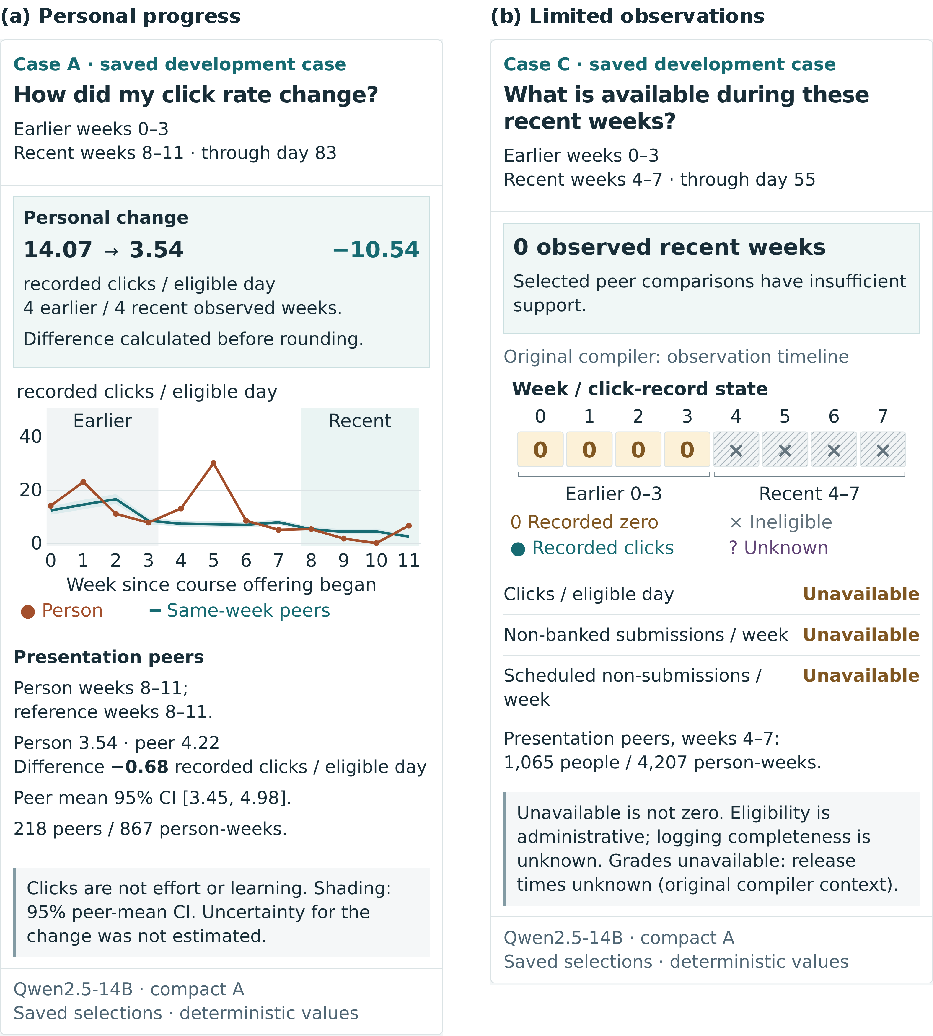
\includegraphics[width=0.9\textwidth]{figures/adaptation.pdf}
\caption{Saved compact-A answers. (a) Case 01: personal change and recent peer context; change uses unrounded means. Shading gives pointwise 95\% bootstrap intervals for peer means, not personal change. (b) Case 09: zeros, ineligibility, and unavailable recent values. Its observation timeline and grade context were compiler supplied; acceptance followed one repair. These examples do not establish educational or usability improvements.}
\label{fig:adaptation}
\end{figure*}

\section{\uppercase{Experiment}}
\label{sec:experiment}
\noindent Four conditions answer identical questions about 24 additional development participants, four per question family. Earlier development established the backend, policy, compiler, and evaluator; its participants are excluded and its results are not pooled here.

\subsection{Cases and Shared Information}
The six families address personal change alongside peers, named reference groups, observation availability, separate personal/peer insufficiency, assessment means with grade context, and alternative periods. Profiles compare weeks 0--3 with 8--11 at day~83, 0--3 with 4--7 at day~55, 0--1 with 2--3 at day~27, 0--3 with 10--11 at day~83, and 2--5 with 6--9 at day~69. Questions specify measure, periods, and cutoff.

Selection uses administrative eligibility and previous attempt status where relevant, never activity magnitudes or model outcomes. Insufficiency cases require fewer than two recent eligible weeks and at least one earlier week. We choose the unused eligible person with the smallest SHA256(seed, case, person), using seed \texttt{stage6-structural-v1-20260918}. All 57 previous and 24 new task participants are excluded from peer pools across registrations. Separate row-based calculations checked 52 fact records; this is computational checking, not human review.

All conditions share questions, family labels, definitions, and interpretation rules. Tasks, prompts, code, sources, settings, scoring, and order were frozen before inference, without subsequent tuning or reruns to obtain success. Hidden facts support only scoring and diagnosis.

\subsection{Conditions and Ablation}
\textbf{Enumeration} follows rules for public families and references using the shared backend, validator, renderer, and six-call limit. Family labels make it a strong baseline for defined tasks, without implying general language understanding.

\textbf{A, compact} selects answer types and returned identifiers, with model-specified support and conclusion scope.
\textbf{B, derived metadata} retains these selections but derives support and scope, uses a neutral heading, and supplies a catalogue of returned answers. B--A tests that combined interface change.
\textbf{C, explicit binding} selects exact analytical identifiers with B's metadata and identical catalogue. C--B tests selection representation; C--A tests the full intervention. No interface supplies hidden requirements or missing comparisons.

\subsection{Model, Budgets and Outcomes}
Agents use Qwen2.5-14B-Instruct \cite{qwenReport,qwenCheckpoint}, revision \texttt{cf98f3b3bbb457ad9e2bb}\allowbreak\texttt{7baf9a0125b6b88caa8}, Transformers 4.55.2, greedy decoding, and BF16 on one RTX~6000 Ada GPU without quantization or offload. Limits are 16,000 input and 1,500 output tokens, six analytical calls, four generations, and one final repair using integrity errors and existing evidence, without completeness feedback. No fallback answers are supplied.

Six A/B/C orderings repeat four times, balancing positions and pair order. All 96 method/case slots ran once; enumeration used the host CPU. An accepted output passes format, scope, support, evidence, numerical, and rendering checks. Complete visible answers additionally satisfy every frozen requirement. Method-selected completeness excludes compiler-only claims, panels, and wording. All cases remain in denominators; optional content earns no automatic credit. The prespecified target required 22/24 complete visible answers, no accepted unsupported quantities, and separate personal/peer answers on all four insufficiency cases. The original comparison was descriptive; Section~\ref{sec:sensitivity} adds post hoc analyses.


\section{\uppercase{Results}}
\label{sec:results}
\noindent Table~\ref{tab:outcomes} retains all 24 cases per condition and is generated from frozen reports. Enumeration answered every question through its own selections. A had the highest frozen agent completeness. These are not newly adjudicated accuracy estimates; Section~\ref{sec:caveat} describes the scoring caveat.

\begin{table*}[!t]
\caption{Frozen outcomes. Every main endpoint retains all 24 cases per condition. ``Selected complete'' excludes compiler-supplied requested answers; enumeration's selections are deterministic. ``Both insuff.'' uses the four cases requesting separate personal and peer insufficiency answers. B's completeness has the answer-form caveat in Section~\ref{sec:caveat}.}
\label{tab:outcomes}
\centering\setlength{\tabcolsep}{4pt}
% BEGIN GENERATED: outcomes
%% Generated from frozen reports; do not edit.
\begin{tabular}{lrrrrr}
\hline
Condition & First valid & Accepted & Visible complete & Selected complete & Both insuff. answers \\
\hline
Enumeration & 24/24 & 24/24 & 24/24 & 24/24 & 4/4 \\
A: compact & 21/24 & 22/24 & 21/24 & 18/24 & 3/4 \\
B: derived metadata & 22/24 & 24/24 & 15/24 & 14/24 & 2/4 \\
C: explicit binding & 21/24 & 21/24 & 15/24 & 11/24 & 1/4 \\
\hline
\end{tabular}
% END GENERATED: outcomes
\space % Preserve the trailing space from the original table input.
\end{table*}


\subsection{Validity, Completeness and Attribution}
B accepted all 24 outputs but had lower frozen completeness than A. Final repairs succeeded in one of three attempts for A, two of two for B, and zero of three for C. No agent met the combined target. Compiler context completed three additional A cases, one B case, and four C cases, without adding comparison/change claims. Disputed B judgments qualify its equality with C.



\subsection{Evidence Retrieval and Failure Mechanisms}
The offline diagnostic found sufficient returned evidence for all 24 questions in both A and B, and 21 in C. In case~15, A nevertheless selected peer comparisons for weeks~0--3 when asked about weeks~10--11. Returned recent evidence supported a separate personal-insufficiency answer, but its peer answer was omitted. Correct earlier window binding does not establish relevance.
Invalid C18--20 analysis batches returned no evidence; final/repair identifiers remained unresolved. No catalogue had been returned, so catalogue contents alone cannot explain these failures. All 168 comparison generations reached end-of-sequence below the output-token limit. Source checks detected no accepted unsupported quantitative answer among 91 accepted dashboards; this establishes agreement with checked fields/support rules, not universal semantic correctness.

\subsection{Unresolved Answer-Equivalence Caveat}
\label{sec:caveat}
B17--20 display both requested recent assessment means within supported personal-change claims. The frozen focal predicate recognizes comparison panels/claims but misses these visible means. B remains 15/24 visible and 14/24 selected complete in the frozen outcomes. Crediting only these four forms gives 19/24 visible complete, below the target; selected completeness stays 14/24 because grade context is compiler supplied. This conditional calculation is not independent adjudication.

C21/C23 display earlier/recent means in peer claims without an explicit personal-change answer; equivalence is a separate question. All 96 slots are prepared for two independent human reviewers and adjudication, but no ratings exist. The requested two-reviewer validation remains outstanding; frozen completeness is not a settled measurement construct.

\begin{figure*}[!t]
\centering
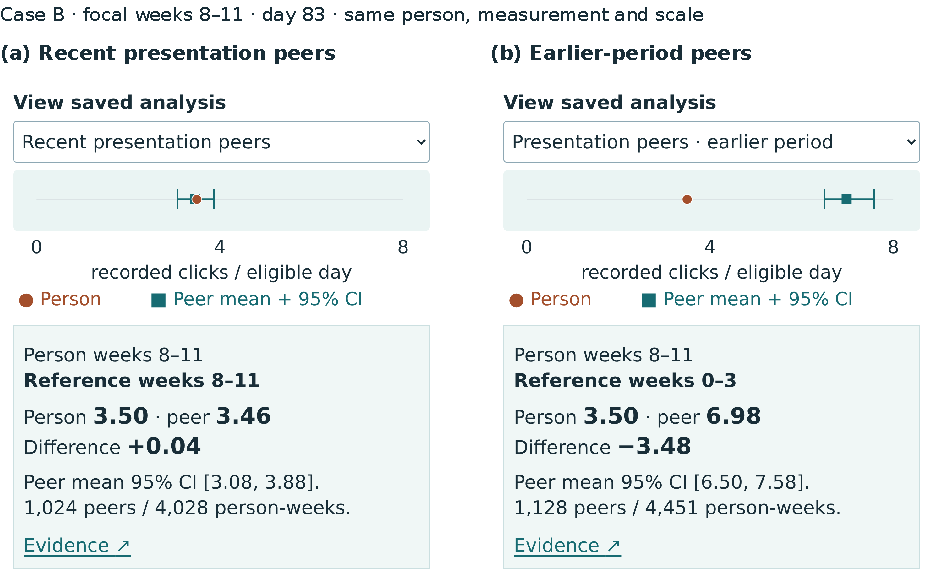
\includegraphics[width=0.9\textwidth]{figures/reference_switch.pdf}
\caption{Saved model-selected comparisons in A05. The focal person, weeks 8--11, units, and scale stay fixed; reference weeks change from 8--11 to 0--3 (1,024 versus 1,128 peers). The selector reads saved results without recalculation. Whiskers are 95\% bootstrap intervals for peer means, not contrasts. Earlier peers are not necessarily fairer or causally adjusted.}
\label{fig:reference}
\end{figure*}

\subsection{Post Hoc Statistical and Data-Quality Checks}
\label{sec:sensitivity}
To address statistical comparison, we applied two-sided exact McNemar tests to paired complete-visible outcomes, with Holm adjustment across all six condition pairs. The unit is the person, not the 96 method/case slots. C--A and B--A each differ by $-25$ percentage points (adjusted $p=0.2813$); C--B differs by zero ($p=1$). Against enumeration, A differs by $-12.5$ points ($p=0.5000$), and B and C each by $-37.5$ points ($p=0.0234$ each). Under the conditional B17--20 credit, B differs from enumeration by $-20.8$ points ($p=0.3125$ after the same six-test adjustment). These exploratory tests assume independent paired cases; shared course/reference pools and structural selection limit inferential interpretation. Non-rejection does not establish equivalence or held-out reliability.

Using preserved features with exact repeated source rows removed, we repeated the numerical comparisons for the same 24 people, profiles, and 81 peer exclusions. Of 52 required feature/reference records, all 29 supported click-rate peer contrasts and all 13 supported personal changes retained their signs. Median/maximum absolute peer-contrast shifts were 0.167/0.324 clicks per eligible day; the maximum personal-change shift was 1.393. All 16 assessment records, support statuses, and eight cross-reference direction conclusions were unchanged. In Figure~\ref{fig:reference}, +0.043 and $-3.480$ become +0.088 and $-3.335$. This post hoc check does not identify unique click events or establish robustness of agent selections. Intervals were not recomputed; no agents were rerun and completeness scores were unchanged.

Across 24 cases, enumeration took 35.40~s, compared with 484.64, 504.21, and 536.32~s for A, B, and C. These descriptive episode totals include failed runs and repairs but exclude shared model loading; enumeration used no inference.

\section{\uppercase{Discussion and Limitations}}
\label{sec:discussion}
\subsection{Lessons for Dashboard Design}
Automatically supplied context can complete an answer without model selection, while B17--20 show that an evaluator can miss equivalent answer forms. Both content and origin therefore matter.

For these structured questions and the small reference registry, the results establish no added agent value over enumeration. A possible role is translating less structured or ambiguous questions into analytical choices when enumerating a larger library is impractical. That role requires a separate comparison using ambiguous questions, clarification behavior, and matched budgets; it was not tested here.

\subsection{Adaptive Views and Operator Context}
In Figure~\ref{fig:reference}, the person's rate stays 3.50 clicks per eligible day while recent and earlier peer means are 3.46 and 6.98, giving differences +0.04 and $-3.48$ before rounding. Periods and membership counts make the reference choice inspectable without implying a preferable or causal comparison.

The graphical trajectories describe recorded activity, not knowledge acquisition. No dashboard intervention or learning-outcome study was conducted, so improvement in students' results or learning cannot be inferred. Grades and banking approval remain unavailable. Effects on operator understanding and usability also require direct evaluation.

\subsection{Scope and Further Validation}
The comparison covers 24 development people from two offerings, with known families and wording and one checkpoint under greedy decoding. Additional independent test cases, preferably reserved people, have not been evaluated. Answer-equivalence judgments should be resolved before locking the system, evaluator, outcomes, and sampling plan for reserved data. A user study should compare interpretation accuracy, completion time, and missing-value/reference errors against a fixed dashboard; no such outcomes are available. New analyses here reuse development cases and do not replace independent validation. Any adjudicated scores should be reported separately from the frozen results.
 OpenAI Codex \cite{openaiCodex} assisted with the programming environment, figure production and language editing.


\section{\uppercase{Conclusion}}
\label{sec:conclusion}
\noindent Across 24 development cases, explicit analytical identifiers did not improve frozen completeness, while enumeration remained complete and cheaper. Correctly calculated values can refer to the wrong period or leave a question partly unanswered, while automatically supplied context can complete an answer without model selection. 
Answer equivalence and measurement choices require review before validation on reserved data. Evaluation should examine operator understanding and usability. 


%\section{\uppercase{AI Assistance Disclosure}}
%\label{sec:disclosure}
%\noindent OpenAI Codex \cite{openaiCodex} assisted with the develop. The experimental model was Qwen2.5-14B-Instruct. Figures depict saved results or programmatic diagrams. The authors retain responsibility for the content.


\bibliographystyle{apalike}
\bibliography{references}
\end{document}
